\chapter{Experimental setup and tests on board}
\section{Test Bench}\label{testbench}
\begin{figure}[H]
	\centering
	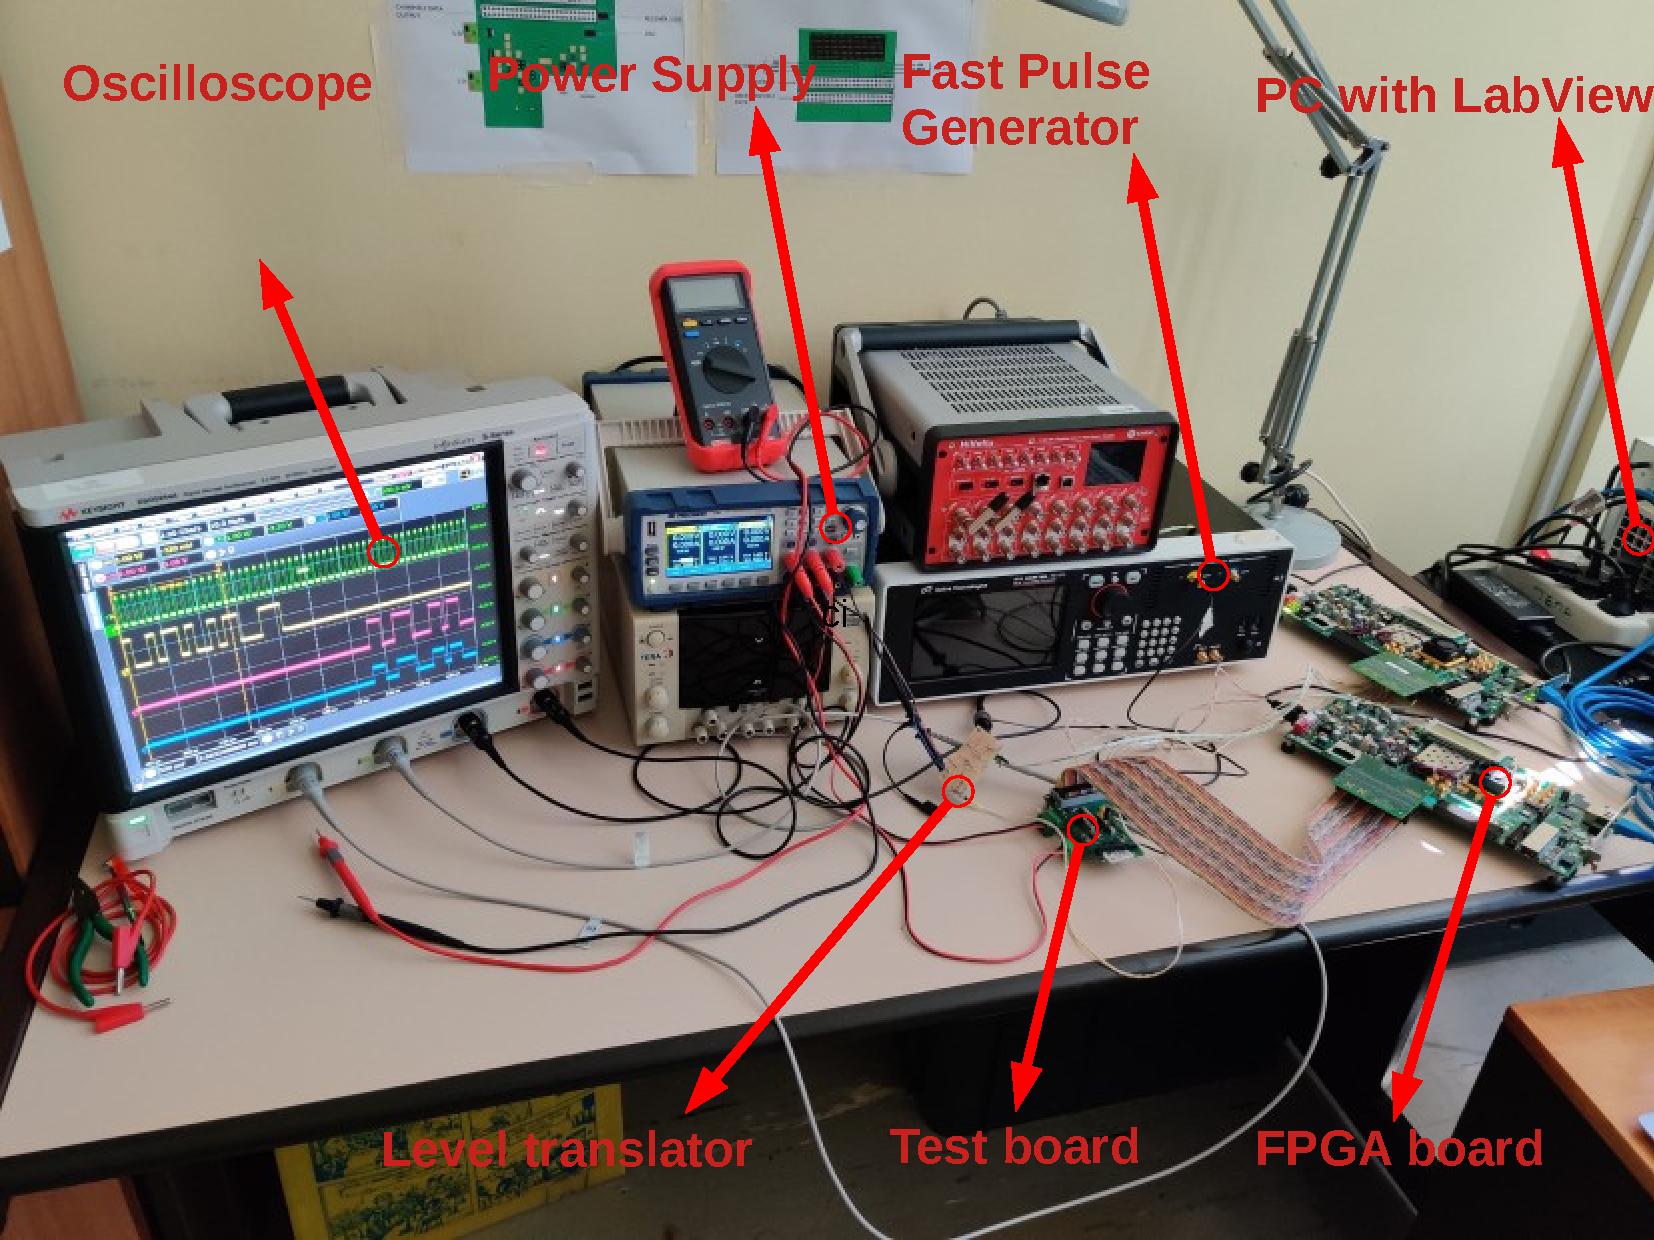
\includegraphics[width=0.7\linewidth]{IMG/ch5/TESTBENCH}
	\caption{test bench setup}
	\label{fig:testbench}
\end{figure}
In order to properly validate the new additions of the FPGA firmware, after the simulations performed in the Vivado design suite, numerous tests have been carried out on the FPGA board and on chip.
The setup used to perform the test is shown in figure \ref{fig:testbench} and it comprehends:
\begin{itemize}
	\item A keysight DSOS254A (Digital Storage Oscilloscope), 4-channels, 2.5~GHz, 20~GSa/s, 10~bit ADC professional oscilloscope
	\item A power supply for the test board and the level translator
	\item A FAst Pulse Generator in order to simulate the signal coming from the detector
	\item A computer with LabView
	\item The FPGA board with the NEW firmware to be tested
	\item The test board with the ABACUS\_v2 bonded to it
	\item A level translator device that will be explained better in section \ref{hardware}.
\end{itemize}

\section{Test board}\label{testboard}
\begin{figure}[H]
	\centering
	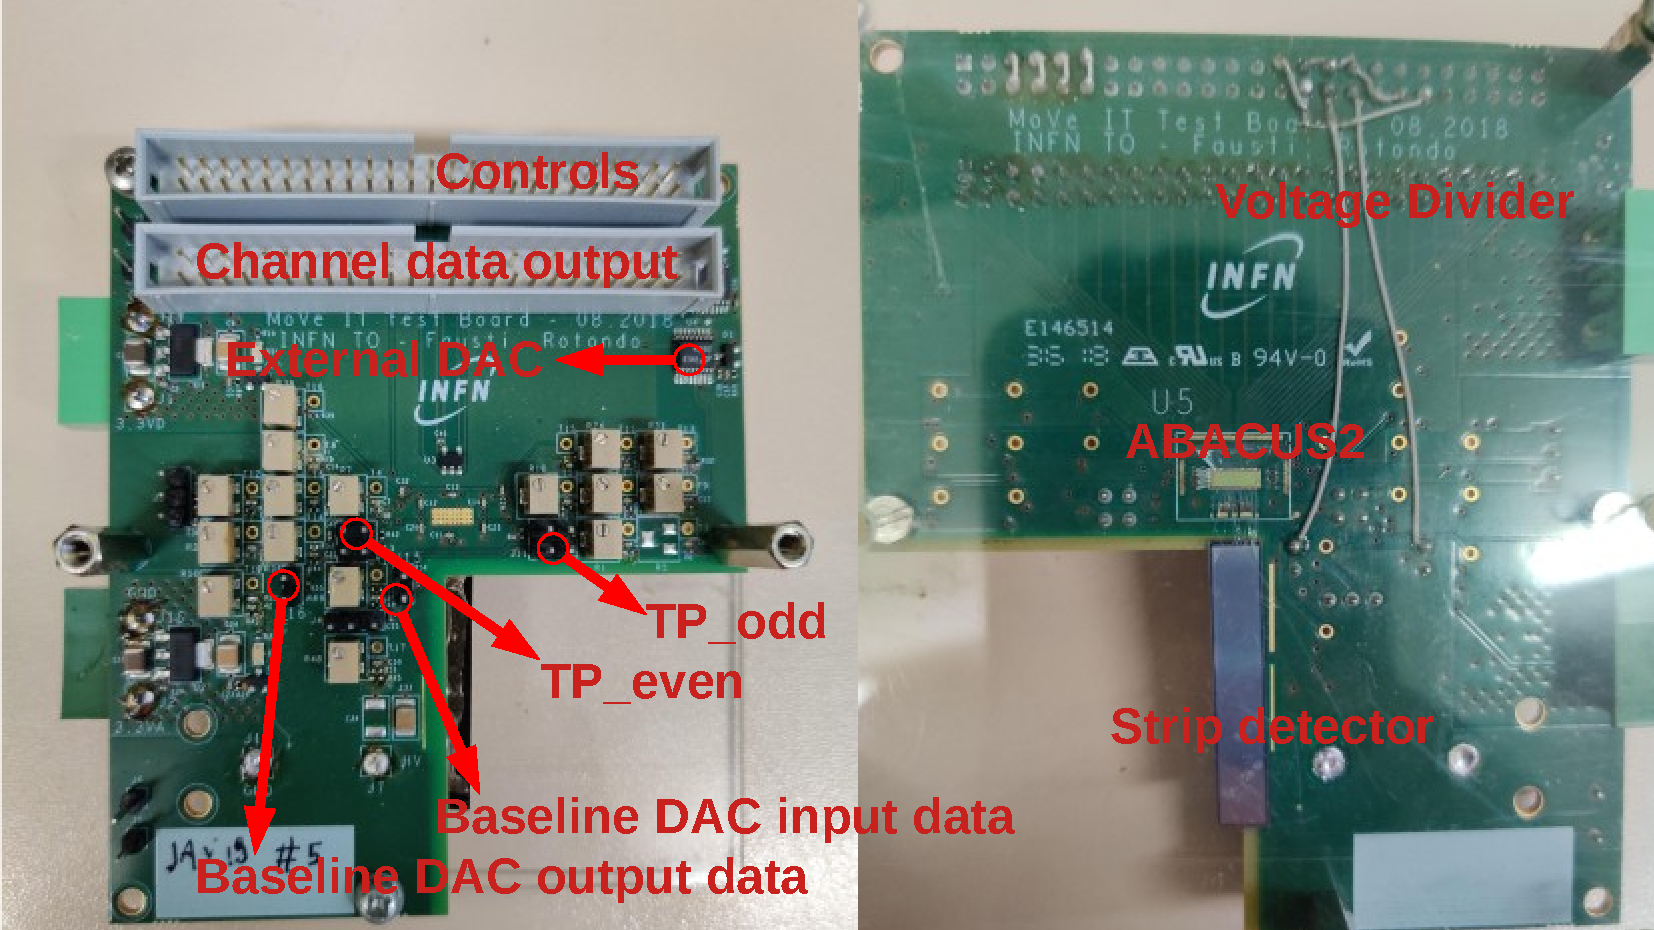
\includegraphics[width=0.7\linewidth]{IMG/ch5/TESTBOARD}
	\caption{test board}
	\label{fig:testboard}
\end{figure}
To test every feature of the ABACUS\_v2 chip the INFN Turin section projected and created a test board shown in figure \ref{fig:testboard}. On the back side of the PCB it can be seen the naked chip bonded to the board. 

\section{Hardware devices}\label{hardware}

\begin{figure}[H]
	\centering
	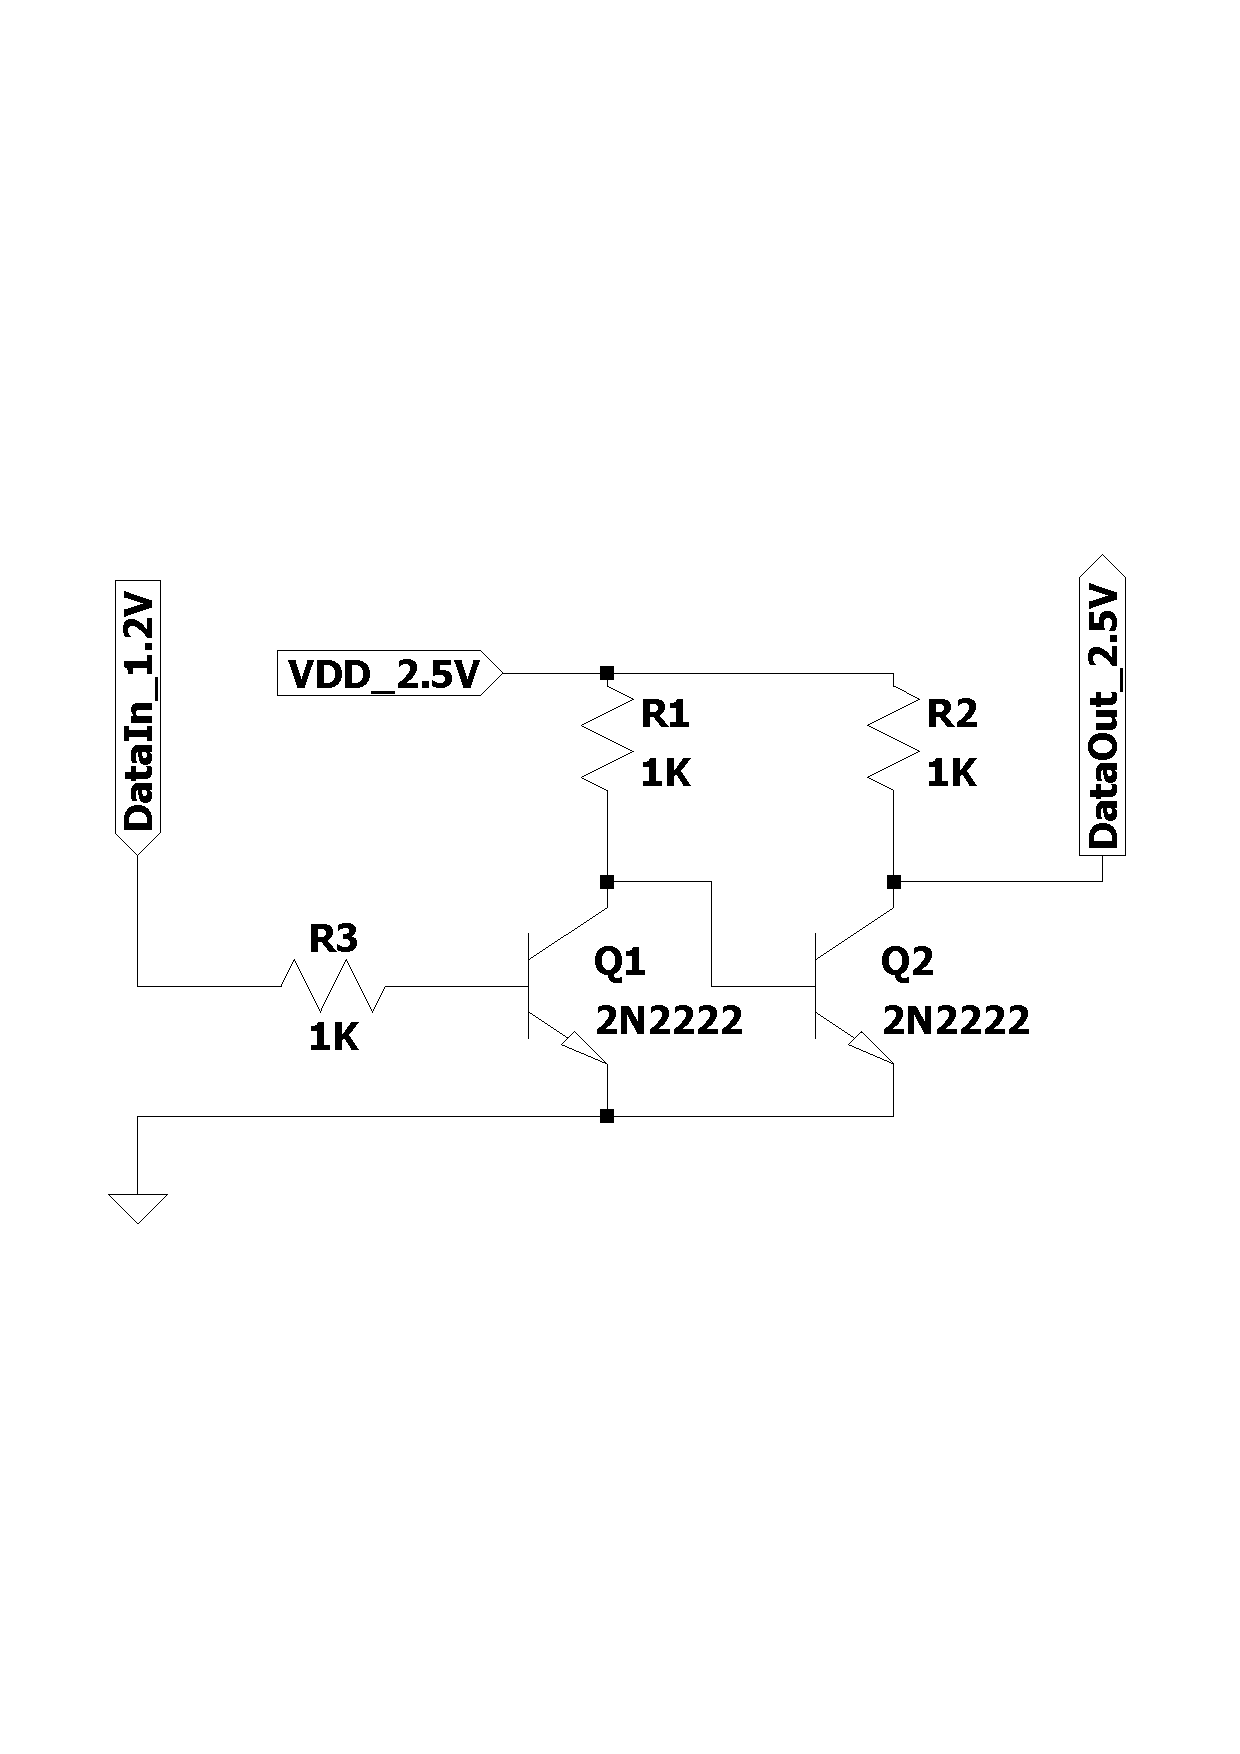
\includegraphics[width=0.7\linewidth]{IMG/ch5/DIAGRAM}
	\caption{test bench}
	\label{fig:diagram}
\end{figure}

\section{Simulations}

\subsection{Internal DAC simulation}\label{dactests}

\begin{figure}[H]
	\centering
	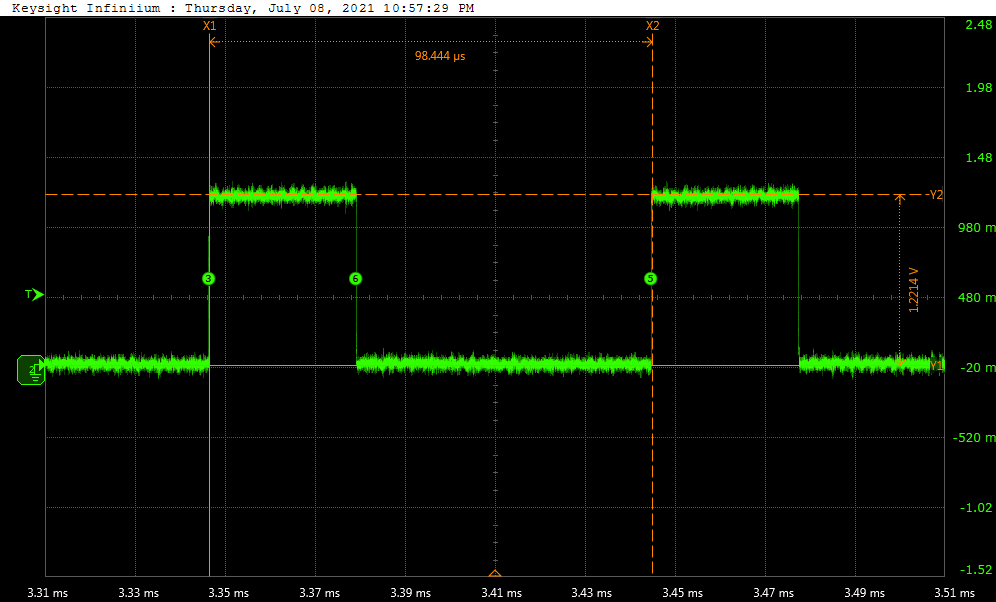
\includegraphics[width=0.7\linewidth]{IMG/ch5/probe/09-08-2021_clock-specks}
	\caption{}
	\label{fig:clockspecs}
\end{figure}


\begin{figure}[H]
	\centering
	\begin{minipage}{.5\textwidth}
		\centering
		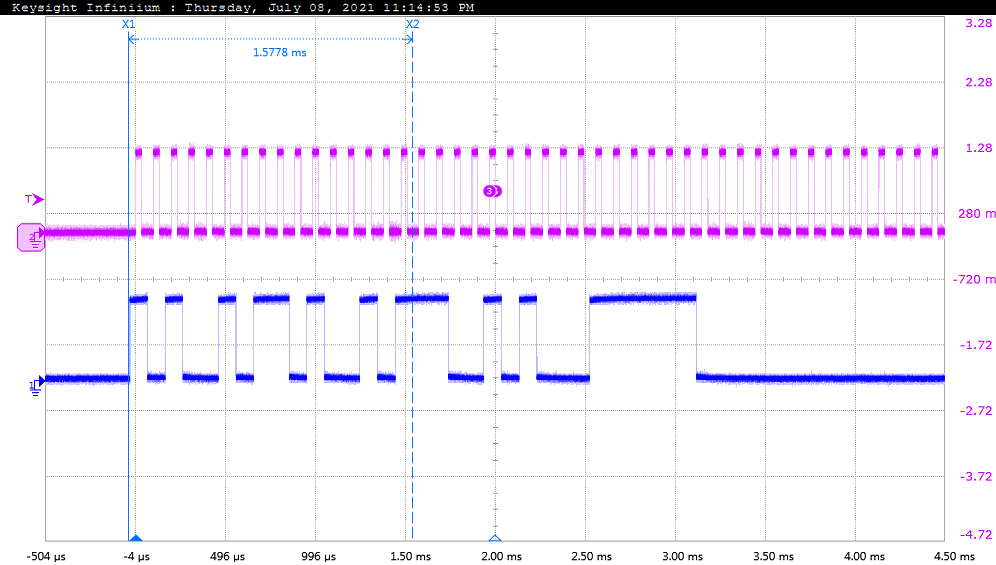
\includegraphics[width=.99\linewidth]{IMG/ch5/probe/09-08-2021_ch05-write63-baselinedac1}
		\caption{}
		\label{fig:ch05write63}
	\end{minipage}%
	\begin{minipage}{.5\textwidth}
		\centering
		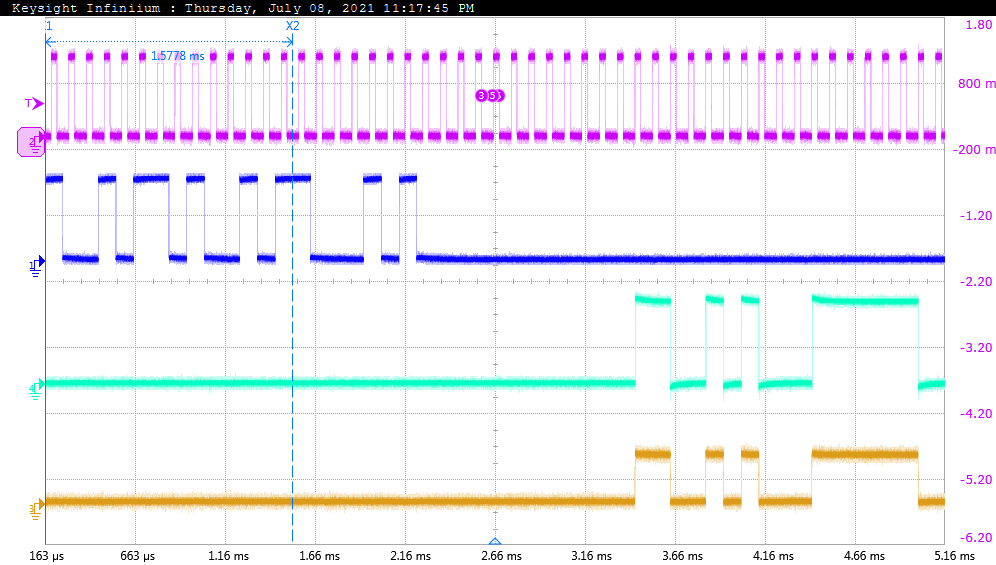
\includegraphics[width=.99\linewidth]{IMG/ch5/probe/09-08-2021_ch05-read63-baselinedac1}
		\caption{}
		\label{fig:ch05read63}
	\end{minipage}
\end{figure}

\subsection{Latching counters simulation}

\subsection{Timestamp generator simulation}

\section{Esa-Abacus}